\documentclass[11pt, oneside]{article}

\usepackage[english]{babel}
\usepackage[utf8]{inputenc}
\usepackage{amsmath}
\usepackage{graphicx}
\usepackage[colorinlistoftodos]{todonotes}
\usepackage{pslatex}
\usepackage[margin=1in]{geometry}
\usepackage{listings}
\usepackage{color}
\usepackage[margin=.25in]{caption}
\usepackage{subcaption}
\usepackage{tikz}
\usepackage{pgfplots}
\usepackage{verbatim}
\usetikzlibrary{automata,topaths}
\definecolor{mygreen}{rgb}{0,0.6,0}
\definecolor{mygray}{rgb}{0.5,0.5,0.5}
\definecolor{mymauve}{rgb}{0.58,0,0.82}

\lstset{ %
  backgroundcolor=\color{white},   % choose the background color
  basicstyle=\footnotesize,        % size of fonts used for the code
  breaklines=true,                 % automatic line breaking only at whitespace
  captionpos=b,                    % sets the caption-position to bottom
  commentstyle=\color{mygreen},    % comment style
  escapeinside={\%*}{*)},          % if you want to add LaTeX within your code
  keywordstyle=\color{blue},       % keyword style
  stringstyle=\color{mymauve},     % string literal style
}


\title{HODOR: HODOR On-Disk Orthogonal Range-trees}

\author{Stephanie Wang (swang93@mit.edu)\\
Bennett Cyphers (bcyphers@mit.edu)\\
Katie Siegel (ksiegel@mit.edu)\\[2ex]
6.851 Final Report}

\date{\today}

\begin{document}

\maketitle
\clearpage

\section{Introduction}

Many web applications today require data queries in two or more dimensions. For instance, a point of interest on a map has latitude and longitude coordinates, and may be indexed by other comparable values. These include start and end times for an event, price ranges for a business, or average user rating for a service. Databases typically support efficient range querying on one primary key at a time. Multi-dimensional range queries, however, are expensive and require several linear passes of the dataset in most implementations. On the other hand, orthogonal range trees with fractional cascading can improve range queries in $d$ dimensions to $O(\log^{d-1} n + k)$ time, where $k$ is the size of the result set [CITATION]. 

In-memory orthogonal range tree implementations have been able to achieve significant query time speedup [CITATION, Tim's paper]. These can be used to extend a database for smaller datasets. Most datasets, however, are too large to fit in memory, and therefore require an on-disk implementation. To this end, we present HODOR, an on-disk Python implementation of range-trees. 

The main obstacle in an on-disk implementation of orthogonal range trees is the added overhead in disk access time. Therefore, in this paper, we explore different methods of optimizing disk I/O accesses. First, we present optimizations on the range tree structure itself. Second, we propose methods of optimizing individual node serialization. Third, we explore optimizing the serialization of the entire tree. Finally, we present results from benchmarking these optimizations against a Python database [BUZHUG CITATION]. 


\section{Data Structure}


Ordinarily, multidimensional range queries are expensive, with most methods taking $O(n)$ time. With large databases, a runtime of $O(n)$ is highly costly. To allow for polylog time range queries, we implemented an orthogonal range tree, generalized to d dimensions. We used a B+ tree for our implementation, as B+ trees are more efficient given the architecture of our machine. In this section, we discuss these data structures and the resulting speedup.

\subsection{B+ Tree-Based Orthogonal Range Tree}
B trees are commonly used for databases, they optimize for the number of disk accesses made for queries. B+ trees are extensions to B trees in which all data is stored in the leaves, and each leaf keeps a pointer to its successor. B+ trees maintain a search time of $O(\log_B n)$. We extend this B+ tree structure to form the orthogonal range tree.

An orthogonal range tree is an extension to a B+ tree in which each node in the tree points to a tree containing the contents of the node's subtree sorted in the next dimension. Dimensions are ordered hierarchically, with the "top level" dimension corresponding to the first-level tree, the second  dimension's information held in subtrees of the nodes in that tree, and so on. B trees support queries in time $O(\log_B^d n + k)$, where $d$ is the number of dimensions of the data. Because we optimize for query time, orthogonal range trees do add a factor of overhead for additional data storage; this space overhead factor is $O(\log_B^{d-1} n)$.   
	
\subsection{Using the data structure}
The tree is constructed in preprocessing, which takes $O(n \cdot \log_B^{d-1} n)$ time. The user can specify any d dimensions for the dataset to be indexed on.
A dimension can be any continuous, comparable data type which can be mapped to a number.
Searches are performed on ranges for any subset of the d dimensions, by passing the range tree a set of {dimension: (range start, range end)} pairs. Open-ended range queries are not explicitly supported, but can be performed in practice by setting one of the range bounds to $\pm\infty$.

\section{Design}

\subsection{Goals}
The main goal of HODOR is to allow efficient range queries of very large
datasets with an arbitrary number of dimensions. We designed the structure to
perform on machines with a limited amount of very fast memory, and a large
amount of memory on a comparatively slow hard disk. As such, we wanted minimize
the time spent reading data from disk, but were generally unconcerned with
in-memory comparison operations. We optimized for this in two ways: first, by
minimizing total disk reads, and second, by chaining consecutive disk accesses
so that they can be executed as efficiently as possible. 

HODOR requires a relatively long time to construct its tree and serialize it
to disk, so the results presented in this paper are for queries on static data
only. In addition, although there have been results for orthogonal range trees
using fractional cascading which achieve $O(\log^{d-2} n)$ query time, we were
most concerned with implementing a working, testable data structure within the
time we had for the project, so we did not attempt to include those techniques
in HODOR.

\subsection{Optimization Methods}
\subsubsection{Range B-Trees}

The standard data structures used for implementing many table-style databases
are the B Tree, and its cousin, the B+ Tree. As a quick overview, a B tree is a
search tree with a branching factor of $B$; i.e., each node points to at most
$B$ children. The logic behind the B tree's design is that, since the act of
loading children from disk into memory is often the bottleneck on database
search performance, each node should load as many children as it can into memory
at once. $B$ can be tweaked to optimize for cache sizes on different machines.
A B-Plus tree is an extension of the B tree in which all data is stored at the
lowest level of the tree (on the ``leaves") and each leaf has a pointer to its
immediate successor leaf. 

Orthogonal range trees were a structure covered in 6.851 which allow $O(\log^d
n + k)$ range queries on $d$ dimensions, where $k$ is the number of data items
returned by the  For HODOR, we extend the B-plus tree
structure with orthogonal, recursive linked trees to create a B-plus Orthogonal
Range Trees (BORT). Each node $n$ in a BORT has a dimension $d$, a set of $B$
child pointers sorted in $d$, and a pointer to another BORT containing all of
the data points contained in $n$'s subtree, known as $n$'s \textit{linked tree}.
When $n$ is loaded into memory, it brings with it all $B$ child pointers and one
link pointer. Therefore, a search on $n$ data points indexed in $d$ dimensions
touches $O(log^d_B n)$ nodes, which requires loading $O(log^d_B n)$ chunks from
disk. However, as we will describe below, not all disk accesses are equal, and
we can achieve better in-practice running times by laying out serialized nodes
intelligently on disk.

\subsection{Node serialization}

In order to store range trees on disk, we require an efficient method to
serialize and deserialize the data structure. In Hodor, we represent a Python
\texttt{RangeTree} instance as a list of serialized nodes, which may be
instances of \texttt{RangeNode} or \texttt{RangeLeaf}. This list is stored in a
``tree file", which can be written to and read by a \texttt{Serializer} class. 

During preprocessing, when building the tree from datapoints,
\texttt{Serializer} is initialized in write mode to build the tree file.
\texttt{Serializer} in write mode exposes a \texttt{dumps(node)} method that
takes in a node instance, serializes the node, and appends it to the tree file.
This method also assigns the node instance a pointer into the tree file, which
is the number of nodes appended previously to it. 

Once the tree is fully built, we call \texttt{Serializer.flush()}, which
flushes the tree file to disk. From this point onwards, \texttt{Serializer} can
be used to read the tree.

In read mode, \texttt{Serializer.loads(pointer)} can be called to deserialize a
single node into a Python node instance, given its pointer into the tree file.
So, to load the child of a node instance, we simply store the child's tree file
pointer as an attribute of the parent. \texttt{loads} is implemented by seeking
the pointer in the tree file and reading out a single node's worth of bytes.

% maybe some of this should go into Implementation details maybe something
% about cPickle vs struct
The seeking method varies by serializer. In Hodor, we test two main node
serialization methods. The first is using a delimiter, such as a newline
character, between nodes. This is convenient because it allows us to support
arbitrarily sized datapoint values. In addition, Python is able to perform
specific line reads quickly, by using either an iterator on the file or a
linecache [CITATION, f.lines() iterator, linecache]. 

The second method we use is to pack nodes into fixed-length strings, which we
call ``blocks". Each node in a range tree stores a constant number of values,
including min, max, and child pointers. This allows us to serialize each node
as a block, as long as we know the maximum sizes of these values. The block
method makes seeking efficient because it allows us to calculate exact offsets
between \texttt{Serializer}'s current byte position in the file and a given
node's pointer. However, this method also limits the amount and type of data
that can be stored at each node. 

\subsection{Tree serialization}

\section{Results}

\subsection{Optimality of Serialization}



\begin{figure}[b!]
\centering
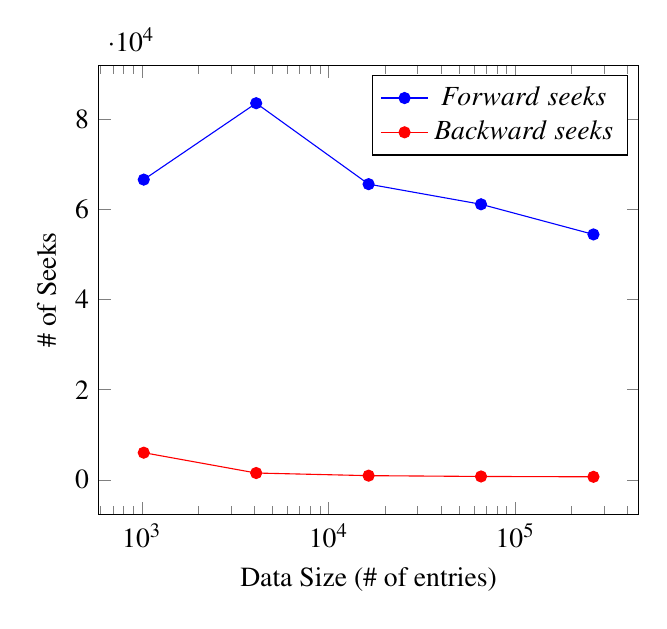
\begin{tikzpicture}
	\begin{semilogxaxis}[
		xlabel=Data Size (\# of entries),ylabel=\# of Seeks]

	\addplot[color=blue,mark=*] coordinates {
		(1024,66681)
		(4096,83658)
		(16384,65676)
		(65536,61205)
		(262144,54509)
	};
	\addplot[color=red,mark=*] coordinates {
		(1024,6022)
		(4096,1504)
		(16384,918)
		(65536,740)
		(262144,664)
	};
	\legend{$Forward\ seeks$,$Backward\ seeks$}
	\end{semilogxaxis}%
\end{tikzpicture}%
\caption{The number of forwards and backwards seeks involved with range queries varies with the size of the data stored in the orthogonal range tree. While backwards seeks are far more costly (10x) than forward seeks, they are far less in number, and decrease with larger data size.}
\label{fig:figure2}
\end{figure}
\subsection{Application to Buzhug Database}
We will now examine the complexity of a search on a fully formed BORT, in terms
of disk reads. The algorithm for searching in a node is as follows, in
pseudocode. Here, \texttt{ranges} is a dictionary of the ranges to be sorted,
indexed by the name of each range's dimension.

\begin{verbatim}

def range_query(ranges):
    start, end = ranges[self.dimension]

\end{verbatim}

\begin{figure}[p]
    \centering
    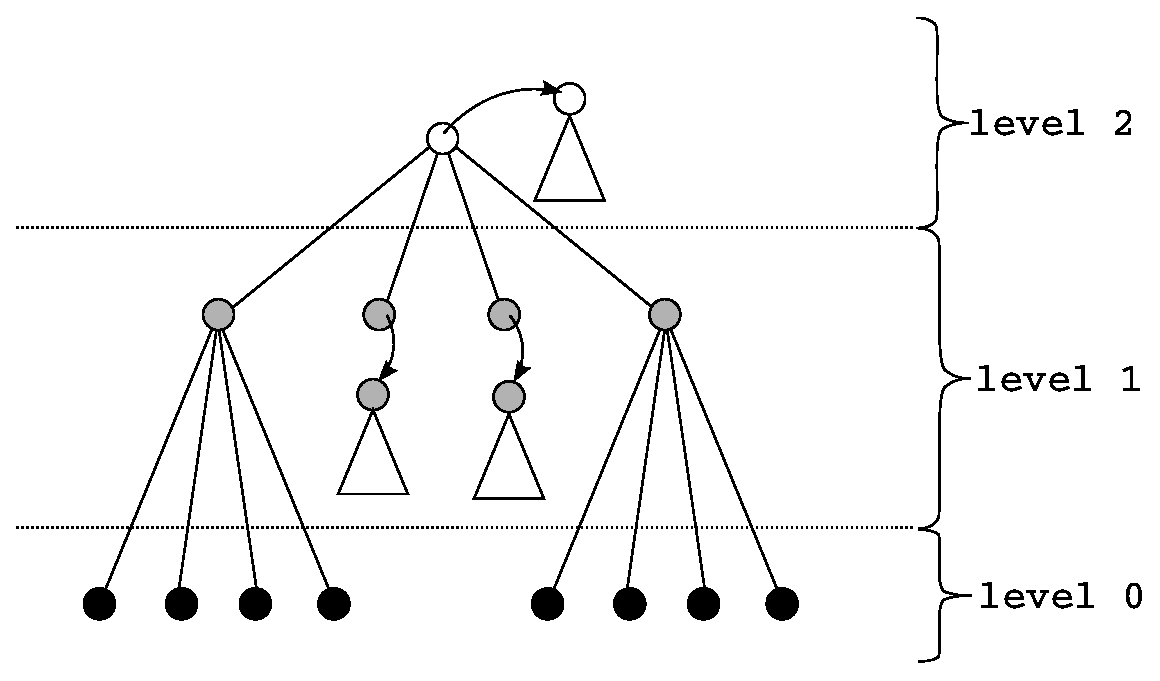
\includegraphics[width=0.8\textwidth]{fig1.eps}
    \caption{Awesome Image}
\end{figure}
\begin{figure}[p]
    \centering
    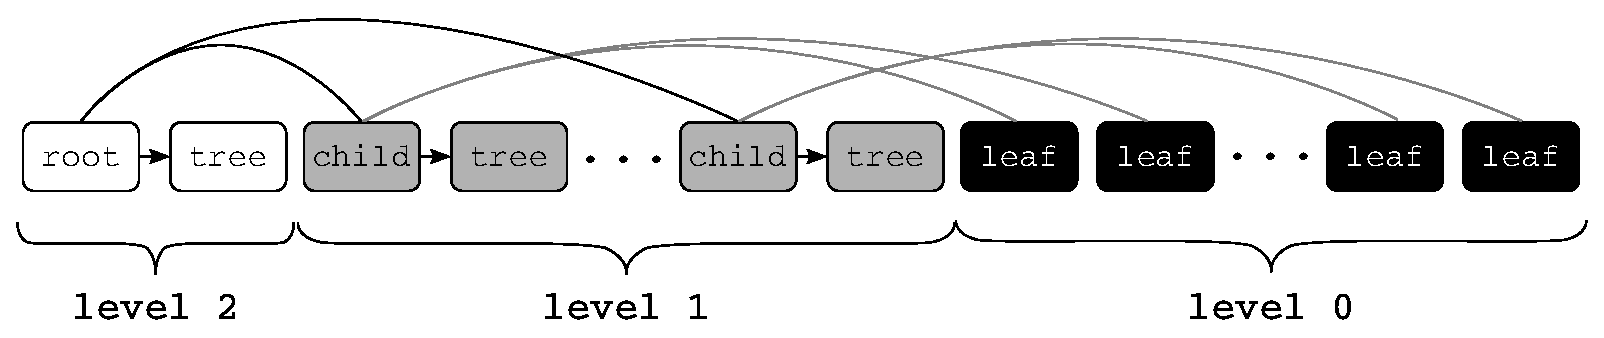
\includegraphics[width=0.8\textwidth]{fig2.eps}
    \caption{Awesome Image}
\end{figure}

\section{Analysis}

We chose to implement HODOR in Python--namely, in conjunction with the Buzhug Python database. Our initial decision allowed for the rapid implementation of the on-disk orthogonal range tree; however, the performance of our database was hindered by our choice of language. As a high-level scripting language, Python does not allow for low-level memory management of data, in contrast to a language such as C. Additionally, inherent aspects of Python such as dynamic typing and a lack of pointer use result in additional overhead. We hypothesize that an implementation of the orthogonal range tree in a low-level language such as C or C++ that allows memory management would allow for faster tree construction and query times. 

A low level language would allow us to specify the exact block size used by the B+ tree on which the orthogonal range tree is built. This block size could be attenuated to the cache block size on the particular machine on which the orthogonal range tree is stored. As such, when a new block is moved into the cache, no space is wasted. Given that queries on the orthogonal range tree move mostly in the forward direction, the proportion of cache hits would increase. Furthermore, nodes could have the same size as the block size optimal for the machine. When the orthogonal range tree is in serialized format, exactly one entire node will be read into the cache at a time allowing for more efficient traversal of the tree structure.

\subsection{BORTs}

\subsection{Optimality of Serialization}

\subsection{Application to Buzhug Database}

An initial goal of our Pythonic implementation of the orthogonal range tree was to integrate the structure seamlessly with an existing Python database--namely, Buzhug. Buzhug is lightweight and stores its data on-disk in in a hierarchical structure. Initial testing of this integration on generated data sets showed that orthogonal range trees are impractical on small data sets. The overhead of generating the tree outweighs any possible performance benefits; ordinary queries are also frequently slower on orthogonal range trees built over small data sets than on the original list of data. However, HODOR is asymptotically less costly than a simple linear search; with larger data sets, such as those found in large data centers, HODOR would likely function comparatively more quickly. Integration of HODOR into large databases--feasible because HODOR stores the orthogonal range tree on disk--would thus be a highly practical implementation scenario.



\subsection{Total Time}

\subsection{Disk Reads}

\section{Conclusion}


\section{References}

\noindent

\begin{description}

\item item

\end{description}
\end{document}
